% $Id: dev_guide1.tex  $

\chapter{Developer's guide}
\minitoc

\section{Introduction}

As described in the Introduction, PRoNTo was developed using a modular structure. There are five main modules (`Data and Design', `Prepare Feature set', `Specify model', `Run model' and `Compute weights') and three reviewing and displaying modules (`Review data', `Review kernel and CV' and `Display results'). This structure not only facilitates the use of the toolbox but also new contributions from developers. These modules have very few dependencies between each other, and for most of them to work, one needs only to provide the `PRT.mat' obtained from the previous module and a few more module specific inputs. This means that the developer can contribute with code for any of the modules without having to adapt the whole toolbox to the changes. Developers can also work only on the module of interest and do not need to be familiar with the functions and sub functions that comprise the rest of the toolbox. In this chapter, we provide a brief description of how the code is organised and how one can contribute with new code, in particular new GUIs and Batch functions. At the end of this chapter, we provide instructions on how to integrate a new machine into PRoNTo. In the current version of PRoNTo, this is the most straightforward extension that can be added. 

\section{Code organisation}

Although from the user's point of view there are five main modules, from the developer's side one can see PRoNTo's functions as belonging to three categories, depending on what they deal with (Figure \ref{Fig1.1}). The first set of functions and sub-functions is responsible for creating PRoNTo's GUIs and matlabbatch menu. The second set of functions comprise all the core routines that implement the machine learning methods (including extraction and preparation of the features, specification and estimation of a model, cross-validation, etc.). The last set of functions correspond to the actual machine learning algorithms that PRoNTo uses for classification and regression. We call these functions the `machines'. The main difference between this last set of functions and the rest, is that one does not need to be familiar with PRoNTo's PRT.mat structure or the rest of the code to be able to integrate a new machine. This can be done very easily, as shown below.

\begin{figure}[!htbp]
  \begin{center}
      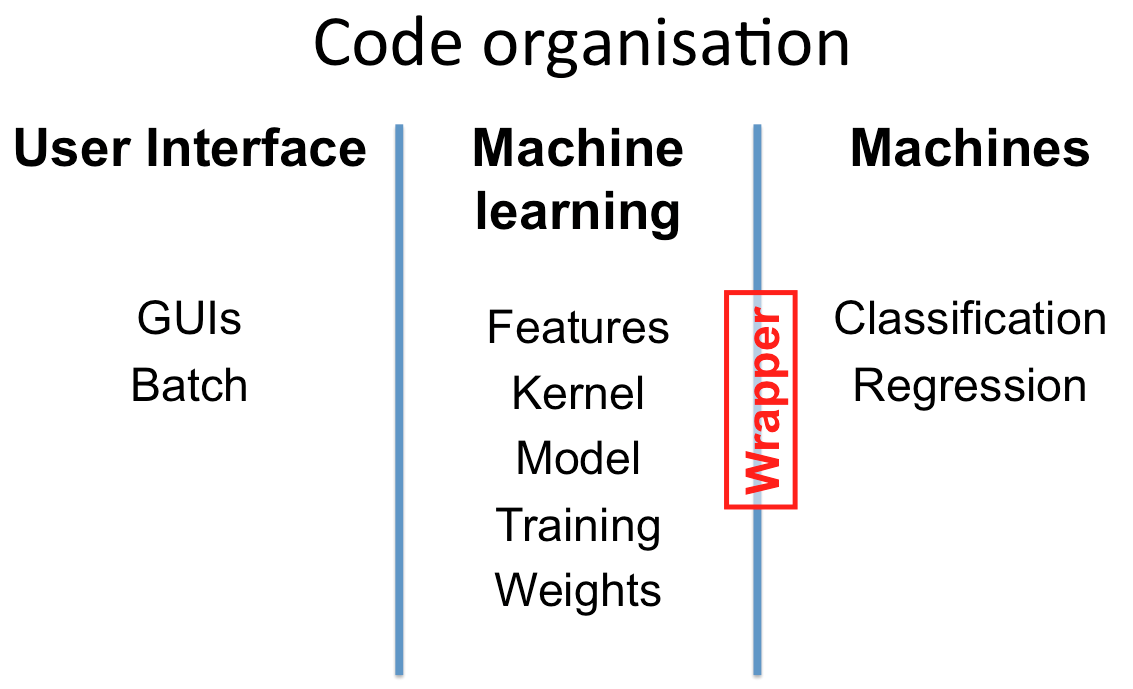
\includegraphics[height=2.2in]{images/code_pronto.png}
   \caption{Organisation of PRoNTo's functions. From the developer's perspective the code is organised in functions and sub functions that deal with the user interface experience (such as GUI and batch functions), the core functions that implement the machine learning approaches (including extracting and preparing the features, specification and estimation of a model, cross-validation routines, etc.) and the actual machine learning algorithms (also known as machines).}
    \label{Fig1.1}
  \end{center}
\end{figure}

\subsection{User interface}

The functions that deal with creating and running PRoNTo's main GUIs have the prefix `prt$\_$ui'. All GUI functions (`.m' files) have a corresponding `.fig' file. This file can be opened and edited using MATLAB's guide functionality. This way one can change the GUI and add extra options to the available menus (for more information, please consult MATLAB's documentation\footnote{http://www.mathworks.com/help/techdoc}).

PRoNTo's matlabbatch functions have either the prefix `prt$\_$cfg', to create a new menu on the batch interface and the prefix `prt$\_$run', to execute instructions using the variables from the corresponding `prt$\_$cfg' function. PRoNTo's batch functionalities work exactly like SPM. For more information on how to contribute with new matlabbatch functions please consult the developer's guide on the SPM8 manual\footnote{http://www.fil.ion.ucl.ac.uk/spm/doc/manual.pdf}.  

\subsection{Machine learning}

The machine learning routines comprise the core of PRoNTo. These routines do most of the necessary instructions to run all machine learning procedures currently implemented in the toolbox. They don't have a specific prefix but from the name of the .m file it is easy to find out what the function does (e.g. prt$\_$compute$\_$weights.m deals with creating new weights images). Most of the functions take as input the PRT.mat structure. Therefore, knowledge of this structure (see next chapter) is required in order to contribute with new code. In the future, we intend to make the process of introducing new feature selection algorithms and other model functionalities as easy as implementing a new machine, as described below.

\subsection{Machines}

Integrating a new machine algorithm, i.e. classifier or regressor, into the PRoNTo framework is straightforward. PRoNTo provides a function called `prt$\_$machine.m' that works as a wrapper around the different machine learning algorithms (functions with prefix `prt$\_$machine'). In brief, this wrapper translates PRoNTo's structure and internal variables into the required inputs for each machine. This way, the machine function needs only to read a simple input format that does not depend on knowledge of how PRoNTo works or of the PRT.mat fields (Figure \ref{Fig1.2}).

\begin{figure}[!htbp]
  \begin{center}
      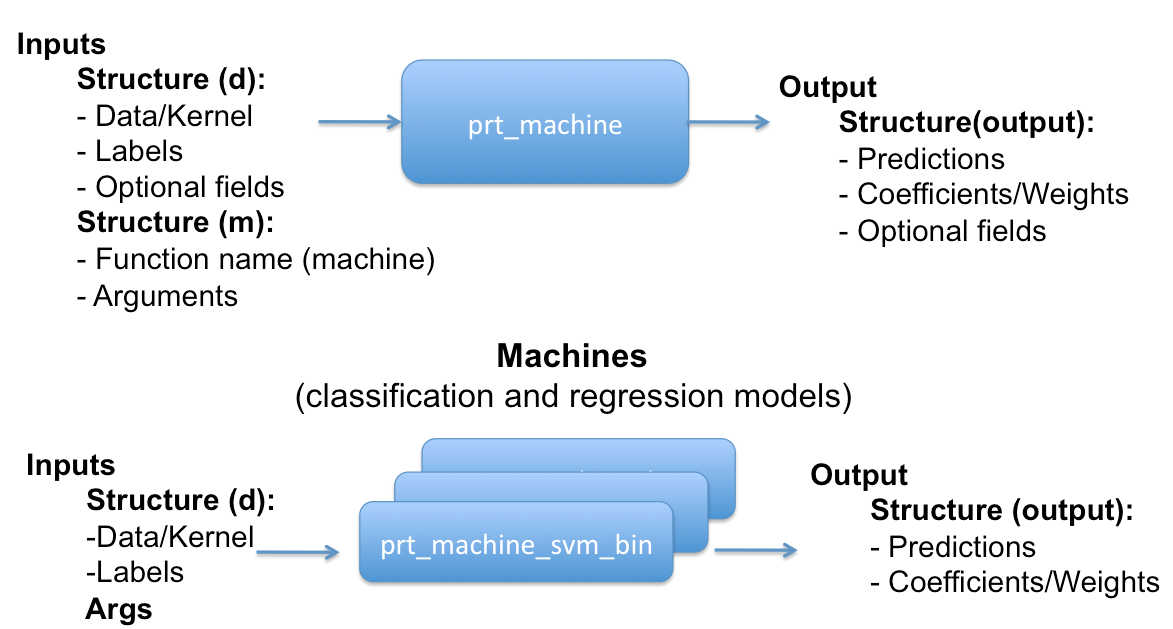
\includegraphics[height=3.0in]{images/machines.png}
   \caption{Code organisation for integrating a new machine with PRoNTo. `prt$\_$machine.m' works has a wrapper that translates PRoNTo's inputs into the machine format inputs and performs extensive error checks on these variables. The machines (such as `prt$\_$machine$\_$svm$\_$bin.m') perform the classifier/regression algorithms and have inputs and outputs that are not dependent on PRoNTo's internal structures.}
    \label{Fig1.2}
  \end{center}
\end{figure}

More specifically, to contribute with a new machine the developer needs to provide a matlab function, which reads the following input data structure, \textit{d}, and optional arguments, \textit{args}, (all fields are mandatory except where otherwise stated):

\begin{itemize}
\item \textit{d} - data structure with input to the classifier/regressor: \\
     \textit{.train} - training data (cell array of matrices of row vectors, each [Ntr x D]). Each matrix contains one representation of the data. This is useful for approaches such as multiple kernel learning. Ntr is the number of training examples and D is the dimension of the feature set (e.g. number of voxels).\\
     \textit{.test} - testing data  (cell array of matrices row vectors, each [Nte x D]). Nte is the number of testing examples and D the dimension of the feature set.\\
     \textit{.tr}$\_$targets - training labels (for classification) or values (for regression) (column vector, [Ntr x 1]).\\
     \textit{.use$\_$kernel} - flag: is data in form of kernel matrices (true) of in form of features (false)?
\item    \textit{args} (optional) - anything else that is specific to the algorithm (e.g. LIBSVM arguments).
\end{itemize}


\begin{figure}[!htbp]
  \begin{center}
      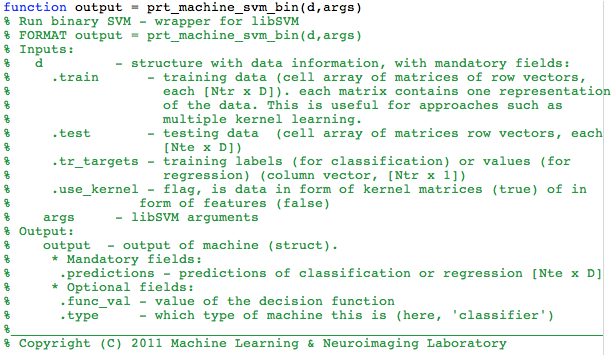
\includegraphics[height=3.0in]{images/prtmachinesvmbin.png}
   \caption{`prt$\_$machine$\_$.m' function help. Example of a PRoNTo machine for 2-class SVM classification.}
    \label{Fig1.3}
  \end{center}
\end{figure}

In addition, the outputs of the function need to have the following format, so that they can be read by the wrapper and translated back to the PRoNTo framework (all fields are mandatory except where otherwise stated) (Figure \ref{Fig1.2}):

\begin{itemize}
\item \textit{output}  - output structure with fields:\\
\textit{.predictions} - predictions of classification or regression [Nte x D]. Nte is the number of test examples and D the dimension of the feature set.\\
\textit{.func$\_$val} (optional) - value of the decision function (if it applies).\\
\textit{.type}  (optional) - type of machine (string: `classifier' or `regressor').
\end{itemize}

The rest of the function can be designed entirely as the developer wishes. The last thing to have in mind is the name of the function itself. It needs to have the prefix `prt$\_$machine' (e.g. `prt$\_$machine$\_$svm$\_$bin' is a function that implements support vector machine binary classification by calling the LIBSVM library). Importantly, the cross-validation and performance measures are performed outside in the main PRoNTo framework, and therefore the machine function should provide only the necessary instructions to implement the classifier/regressor algorithm.

Finally, the new machine is easily integrated with PRoNTo by including the name of the file in the corresponding GUI and Batch functions (prt$\_$ui$\_$model.m and prt$\_$cfg$\_$model.m, respectively).

The same procedure applies to the weights functions. PRoNTo provides a wrapper function called `prt$\_$weights'. The procedure for integrating a new weights function is exactly the same as for a new machine.

Both wrapper functions, `prt$\_$machine' and  `prt$\_$weights', perform extensive tests to make sure the machines and weights code complies to the specific inputs and outputs required by the framework. 







